\subsection{Basic Algorithm}

The basic algorithm connects interested peers with one another via a Distributed Hash Table (DHT).

The DHT is formed by running an instance of the Bamboo OpenDHT code on approximately 1000 PlanetLab peers\footnote{Typically only about 300 are stably active.}.  
3 peers are designated as ``gateways" that the others contact to ``bootstrap" themselves into the DHT.  After servers join the DHT, each 
creates a web service that accepts queries from peers outside the DHT.  When a server receives a
query, it forwards it through the DHT, retrieves the answer, and returns the answer to the requestor. The DHT is only used to store only peer information, 
to connect peers downloading the file to each other.
Data is stored as key, value maps, with many values storable per key.  If there are more than ten values stored, only the first 10 values are returned for the first request. 
If a peer wants the rest of the values, it must make a repeat query and request values 11-20, etc.  Members of the DHT run continously, servicing requests.

In order for our peers to then use this DHT, each is given a list of all known DHT members out-of-band.  When they are instructed to download a file, 
they ``port sniff" on the web service ports of known DHT members, to create a local list of live DHT members.  They query 10 DHT servers at a time, until they have found at least 5 that are active.
They then round robin across the list of known active proxies for queries they perform.

When a peer performs a query, for example for a key ``file x block y", it requests this key and also a ``redundant key" for the same, 
like ``file x block y copy 1".  It requests both keys from 2 different gateways (using the round robin described above), 
thus the total number of queries per request is 4.  
The reason it does this is that sometimes keys are hosted by poorly connected members of the DHT, so are slow, and so duplicate keys avoids this slowdown.
Sometimes gateways themselves are temporarily slow, so using multiple gateways per request avoids this slowdown, as recommended by the authors of opendht \cite{opendht_embarrassing}.

A peer wishing to download a file first tries to download it from the origin web server using traditional client-server download.  
If at some point one of the following conditions occurs, the client switches to using 
peer-to-peer delivery:
\begin{enumerate}
\item First, the client waits a maximum number of seconds $T$ after the start of a download, to receive the first byte of data from the origin server.  
First data byte means any byte received from the origin--a header or content byte.  TCP connection handshake packets do not count as a data byte.
If $T$ seconds pass without the client receiving any data, it transitions to a peer-to-peer delivery.  This allows the system to decide quickly whether the origin server is over-burdened.   
\item After the client begins receiving data from the server, it monitors whether the download rate falls below a certain 
threshold of $R$ bytes per second over the last $W$ seconds.  It starts measuring this after the first byte is received.  
If the receive rate ever drops below $R$, the client transitions to peer-to-peer delivery.  
This is to accomodate servers with slow connections or servers that become overloaded during a download.
\end{enumerate}

If a client transitions to peer-to-peer delivery, it first checks to see if it knows enough meta-data for the file it is downloading (it needs to know the size in order to look up peer lists).
If the client has previously received a TCP header with size information from the origin, it has the information it needs.  If it doesn't, it
queries the DHT (using a key of the url being downloaded) for known meta-data that other peers will have placed there when they previously downloaded the file.  While performing
this DHT lookup, it also does an HTTP HEAD 
request for the file to the origin server, and uses the response from either of these two to determine file size.  
If there is no meta-data listed in the DHT, it continues to poll the DHT every 5 seconds to see if meta-data for the file has appeared.  At some point
either the meta-data will appear in the DHT or the HTTP HEAD request will return (with size information) and the peer will then have the meta-data it needs and will start the peer-to-peer
delivery.

To accomplish peer-to-peer delivery, the peer randomly chooses $b$ (undownloaded) blocks of the file to download at a time.  
It retrieves the list of peers who have each block by querying the DHT using a key composed of
the URL concatenated with a given block number, thus finding an associated peer list.  
If there are no peers listed yet for that block, it polls the DHT every 1s to see if new peers have recently added themselves to the list.
While it does not yet have a list of peers, it also contacts the origin and starts a download of the block, so as to 
not waste time in the case that no peers are ever available.  This is useful for some peers that have DHT connections that are too slow.
When it receives a peer list (which includes the first 10 peers in the list), it shuffles that list of 10 peers randomly, then connects to each peer one at a time, and requests the block.  
If the peer beings to serve the block, the peer closes any connections to the origin (if any), and downloads the rest of the block from that peer.  If the peer interrupts the connection
or is not online, it chooses the next peer until it runs out of peers to use.  Then it repeats the steps for that block, but requesting the next 10 peers listed in the DHT.

We set DHT requests to timeout after 60 seconds if no response is received, as a reasonable value to keep from 
overloading the DHT.  When a request times out, we automatically retry it, for up to 3 times, before giving up on the request.

When a peer only has a few blocks remaining, it tries to download the last few blocks from several peers (redundantly), in an effort to avoid the last block problem \cite{last_block}.  
It downloads all remaining blocks from a total of $b$ peers, so if $b$ is set to 6 and 3 blocks are left, it downloads each remaining block from 2 redundant peers, with the
last block being downloaded from all $b$ peers redundantly.

After completing its download of a block, the peer adds itself to the list of peers willing to share that block (Fig. \ref{fig:download_all_steps}). 

While downloading a file, when a peer first learns the size of the file (via its original HTTP request or its HTTP HEAD request), it stores this ``meta-data" about the file
in the DHT.  It does this by querying to see if this data has already been stored there.  If it hasn't, it stores it by setting the value of the URL in the DHT to the file's size. 
Later peers then use this to retrieve the meta-data for the file if necessary.

After completing a download, the peer lingers a certain number of seconds.  After its linger time is up, it drops all current connections to peers, and performs DHT remove requests to
remove itself from the peer lists in the DHT.

\begin{figure*}
  \begin{center}
    \subfigure[Peer downloads meta-data]{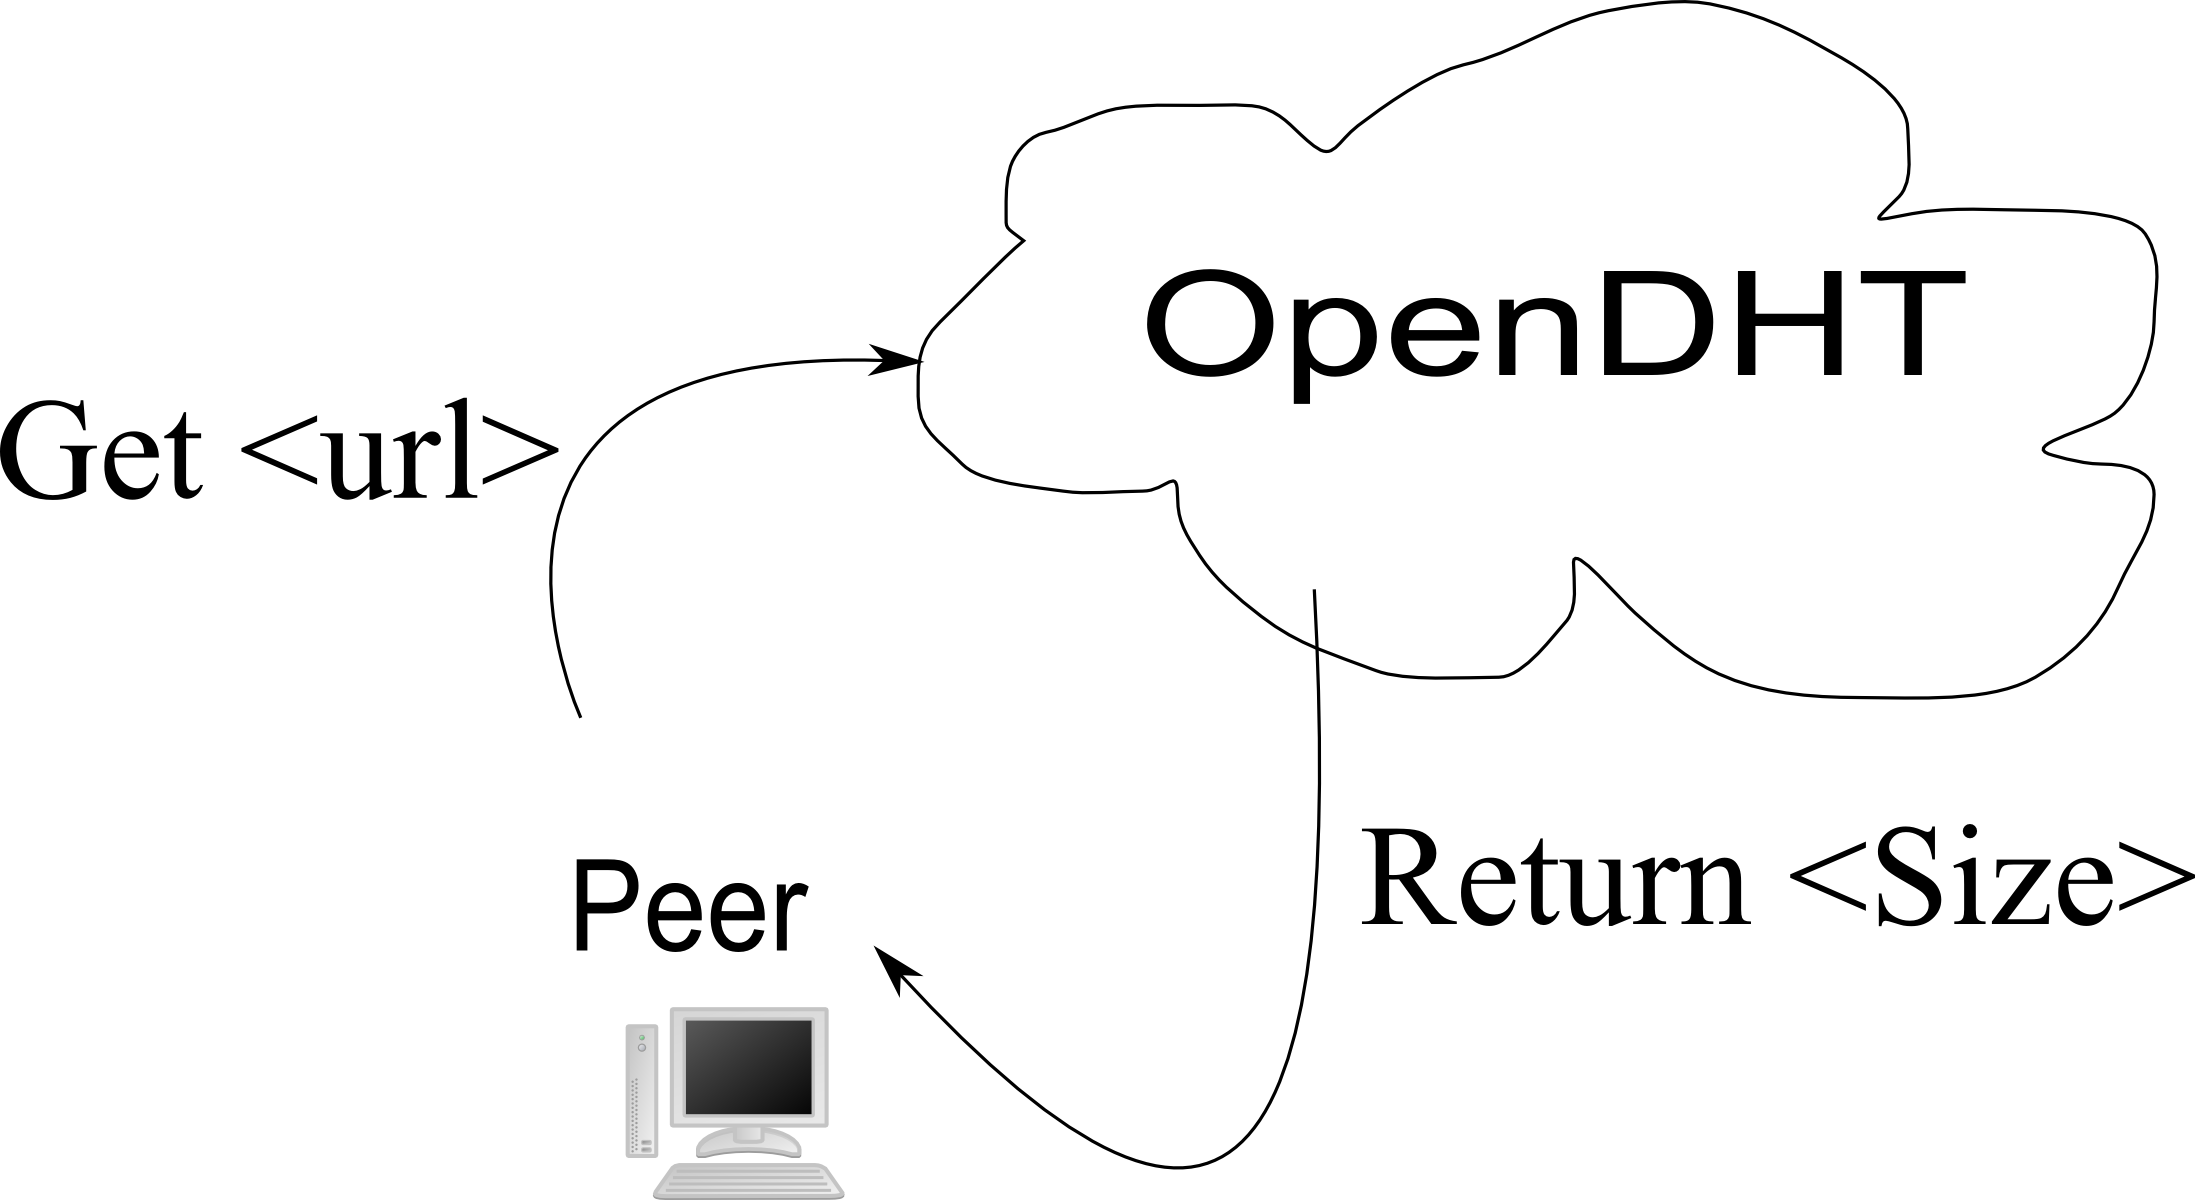
\includegraphics[width=7cm]{description_pics/peer_step_1.png}}
    \subfigure[Peer downloads a list of peers that have a block]{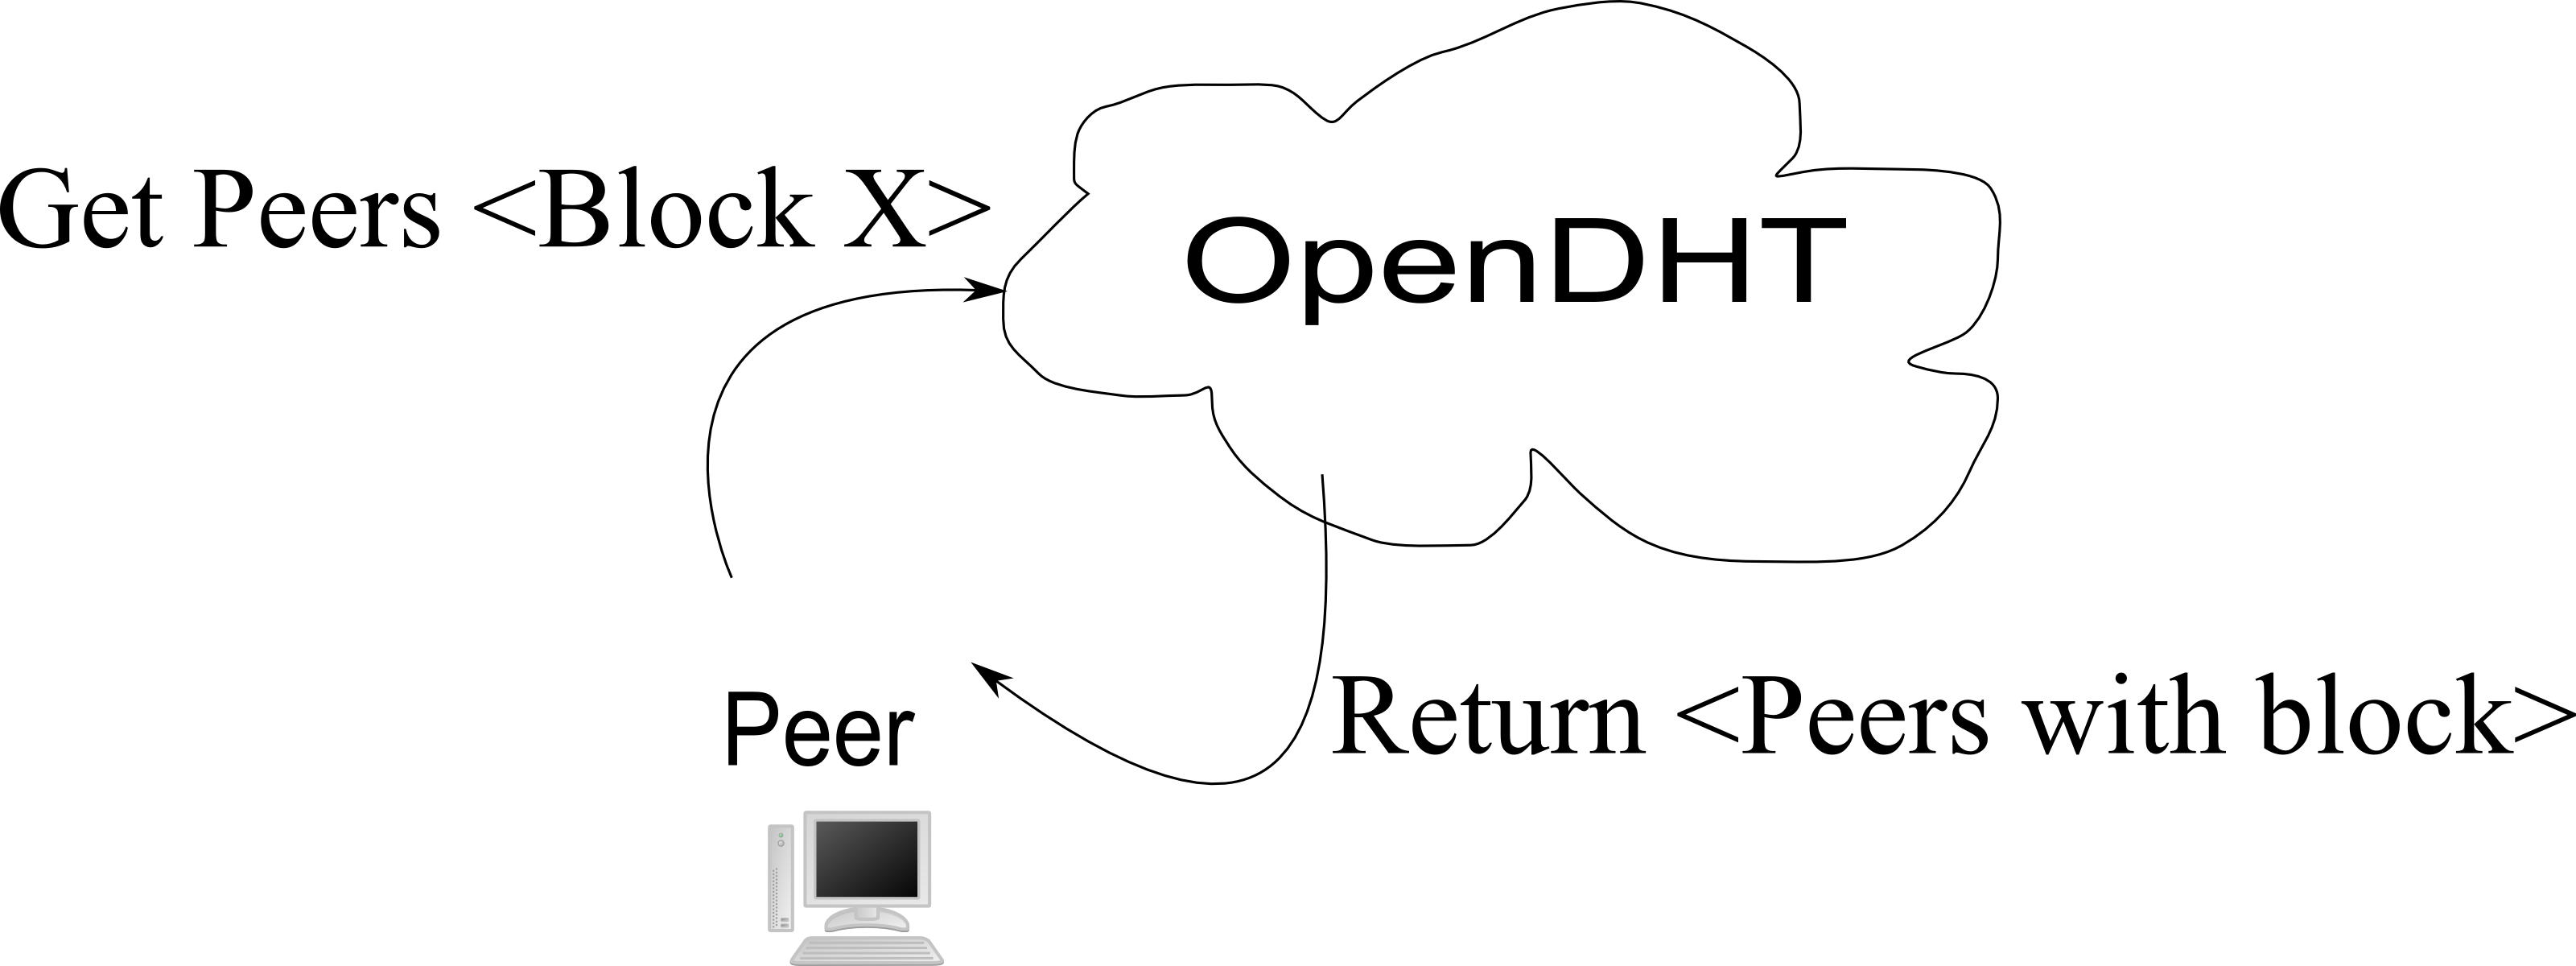
\includegraphics[width=10cm]{description_pics/peer_step_2.png}}
    \subfigure[Peer adds itself to list of peers who have the block]{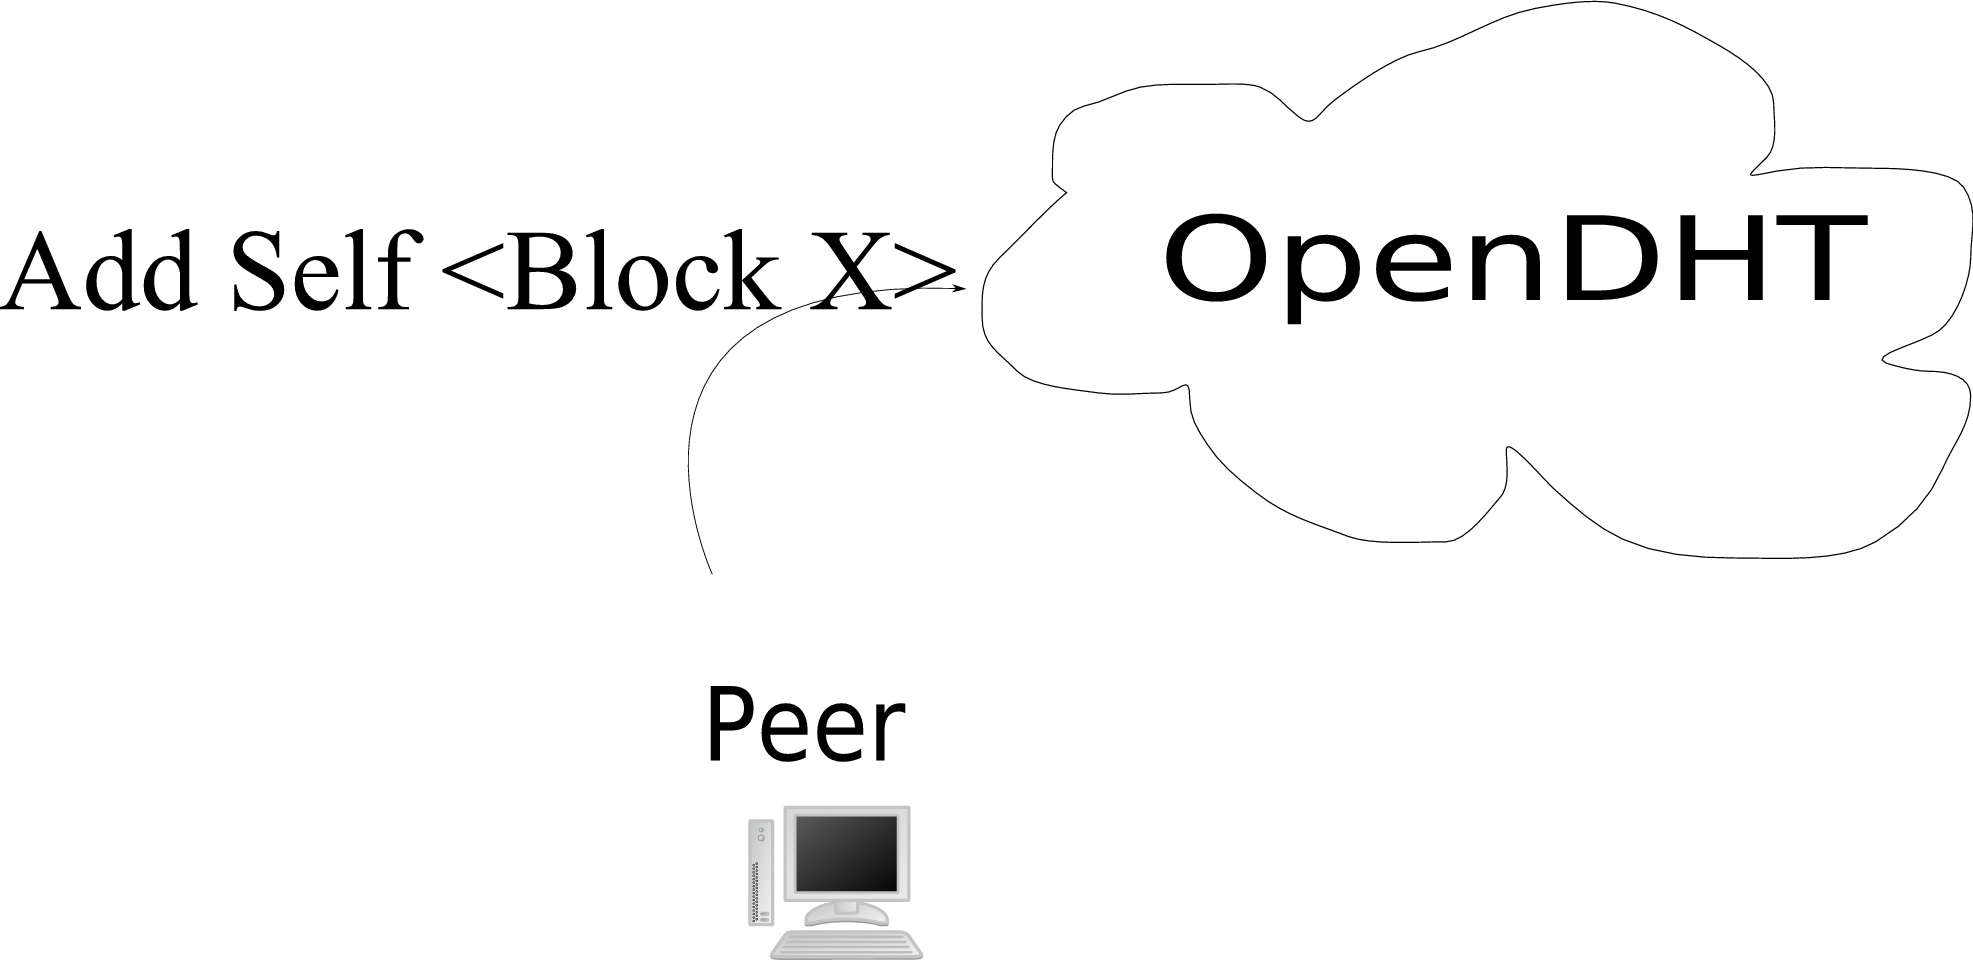
\includegraphics[width=8cm]{description_pics/peer_step_3.png}}
    \caption{Steps to accomplish a peer-to-peer-web download}
    \label{fig:download_all_steps}
  \end{center}
\end{figure*}

